\documentclass[12pt,letterpaper]{article}
\usepackage[T1]{fontenc}
\usepackage{tgheros}
\renewcommand{\familydefault}{\sfdefault}
\usepackage[letterpaper, left=0.75in, right=0.75in, top=0.85in, bottom=0.85in,
  headheight=16pt, headsep=14pt, footskip=26pt]{geometry}
\usepackage{fancyhdr}
\usepackage{pifont}
\usepackage{tikz}
\usetikzlibrary{arrows.meta}
\pagestyle{fancy}
\fancyhf{}
\fancyhead[L]{Week NN / Train-yard sorting / Grades 4–5}
\fancyfoot[L]{\small Bellingham Math Circle / Week NN / TY-45-v1}
\fancyfoot[R]{\small \thepage}
\renewcommand{\headrulewidth}{0.4pt}
\renewcommand{\footrulewidth}{0pt}
\setlength{\parindent}{0pt}
\setlength{\parskip}{4pt}
\newcommand{\problem}[1]{\par\vspace{14pt}\noindent\textbf{Problem #1:} }
\newcommand{\yes}{\ding{51}}
\newcommand{\no}{\ding{55}}
\begin{document}

Put a train on the arrival track exactly as it is drawn, so the car on the left arrives first. Each move sends the front car of the arrival track down into the siding, or sends the top car of the siding out to the departure track. Cars slide along the table and never jump over each other. A car in the siding cannot go back to the arrival track. A train can \emph{leave in order} if its cars can reach the departure track in the order 1, 2, 3, and so on. For trains with more than five cars, make extra cars from paper squares, and pretend the siding is long enough to hold every car.

\par\vspace{2pt}\begin{center}
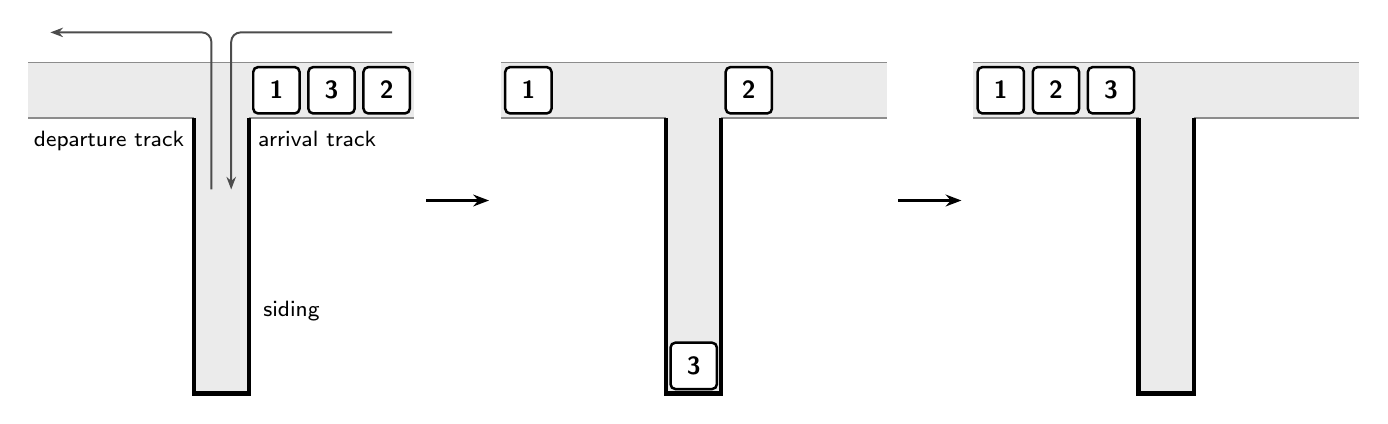
\begin{tikzpicture}[x=1mm,y=1mm]
\begin{scope}[shift={(21,0)}]
\fill[black!8] (-21,0) rectangle (28,7);
\fill[black!8] (0,-35) rectangle (7,0);
\draw[black!45, line width=0.5pt] (-21,7) -- (28,7);
\draw[black!45, line width=0.5pt] (-21,0) -- (0,0);
\draw[black!45, line width=0.5pt] (7,0) -- (28,0);
\draw[line width=1.6pt] (0,0) -- (0,-35) -- (7,-35) -- (7,0);
\draw[line width=0.9pt, fill=white, rounded corners=0.6mm] (7.56,0.56) rectangle (13.44,6.44);
\node at (10.5,3.5) {\bfseries\small 1};
\draw[line width=0.9pt, fill=white, rounded corners=0.6mm] (14.56,0.56) rectangle (20.44,6.44);
\node at (17.5,3.5) {\bfseries\small 3};
\draw[line width=0.9pt, fill=white, rounded corners=0.6mm] (21.56,0.56) rectangle (27.44,6.44);
\node at (24.5,3.5) {\bfseries\small 2};
\node[font=\footnotesize, below left, inner xsep=1pt] at (-0.8,-0.4) {departure track};
\node[font=\footnotesize, below right, inner xsep=1pt] at (7.8,-0.4) {arrival track};
\node[font=\footnotesize, right] at (7.6,-24.5) {siding};
\draw[-{Stealth[length=1.6mm]}, line width=0.7pt, black!70, rounded corners=1.2mm] (25.2,10.85) -- (4.76,10.85) -- (4.76,-9.1);
\draw[-{Stealth[length=1.6mm]}, line width=0.7pt, black!70, rounded corners=1.2mm] (2.24,-9.1) -- (2.24,10.85) -- (-18.2,10.85);
\end{scope}
\draw[-{Stealth[length=2mm]}, line width=0.9pt] (50.5,-10.5) -- (58.5,-10.5);
\begin{scope}[shift={(81,0)}]
\fill[black!8] (-21,0) rectangle (28,7);
\fill[black!8] (0,-35) rectangle (7,0);
\draw[black!45, line width=0.5pt] (-21,7) -- (28,7);
\draw[black!45, line width=0.5pt] (-21,0) -- (0,0);
\draw[black!45, line width=0.5pt] (7,0) -- (28,0);
\draw[line width=1.6pt] (0,0) -- (0,-35) -- (7,-35) -- (7,0);
\draw[line width=0.9pt, fill=white, rounded corners=0.6mm] (-20.44,0.56) rectangle (-14.56,6.44);
\node at (-17.5,3.5) {\bfseries\small 1};
\draw[line width=0.9pt, fill=white, rounded corners=0.6mm] (0.56,-34.44) rectangle (6.44,-28.56);
\node at (3.5,-31.5) {\bfseries\small 3};
\draw[line width=0.9pt, fill=white, rounded corners=0.6mm] (7.56,0.56) rectangle (13.44,6.44);
\node at (10.5,3.5) {\bfseries\small 2};
\end{scope}
\draw[-{Stealth[length=2mm]}, line width=0.9pt] (110.5,-10.5) -- (118.5,-10.5);
\begin{scope}[shift={(141,0)}]
\fill[black!8] (-21,0) rectangle (28,7);
\fill[black!8] (0,-35) rectangle (7,0);
\draw[black!45, line width=0.5pt] (-21,7) -- (28,7);
\draw[black!45, line width=0.5pt] (-21,0) -- (0,0);
\draw[black!45, line width=0.5pt] (7,0) -- (28,0);
\draw[line width=1.6pt] (0,0) -- (0,-35) -- (7,-35) -- (7,0);
\draw[line width=0.9pt, fill=white, rounded corners=0.6mm] (-20.44,0.56) rectangle (-14.56,6.44);
\node at (-17.5,3.5) {\bfseries\small 1};
\draw[line width=0.9pt, fill=white, rounded corners=0.6mm] (-13.44,0.56) rectangle (-7.56,6.44);
\node at (-10.5,3.5) {\bfseries\small 2};
\draw[line width=0.9pt, fill=white, rounded corners=0.6mm] (-6.44,0.56) rectangle (-0.56,6.44);
\node at (-3.5,3.5) {\bfseries\small 3};
\end{scope}
\end{tikzpicture}
\end{center}

\problem{1}Which of these six trains can leave in order? Mark each one \yes{} or \no. How many of the 24 trains with cars 1, 2, 3, 4 can leave in order?
\par\vspace{8pt}\begin{center}
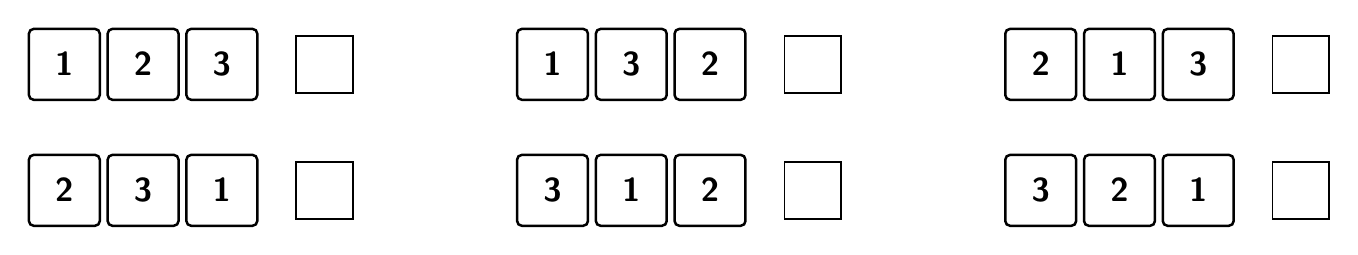
\begin{tikzpicture}[x=1mm,y=1mm]
\draw[line width=0.9pt, fill=white, rounded corners=0.6mm] (0,0) rectangle (9,9);
\node at (4.5,4.5) {\bfseries\large 1};
\draw[line width=0.9pt, fill=white, rounded corners=0.6mm] (10,0) rectangle (19,9);
\node at (14.5,4.5) {\bfseries\large 2};
\draw[line width=0.9pt, fill=white, rounded corners=0.6mm] (20,0) rectangle (29,9);
\node at (24.5,4.5) {\bfseries\large 3};
\draw[line width=0.6pt] (33.95,0.9) rectangle (41.15,8.1);
\draw[line width=0.9pt, fill=white, rounded corners=0.6mm] (62,0) rectangle (71,9);
\node at (66.5,4.5) {\bfseries\large 1};
\draw[line width=0.9pt, fill=white, rounded corners=0.6mm] (72,0) rectangle (81,9);
\node at (76.5,4.5) {\bfseries\large 3};
\draw[line width=0.9pt, fill=white, rounded corners=0.6mm] (82,0) rectangle (91,9);
\node at (86.5,4.5) {\bfseries\large 2};
\draw[line width=0.6pt] (95.95,0.9) rectangle (103.15,8.1);
\draw[line width=0.9pt, fill=white, rounded corners=0.6mm] (124,0) rectangle (133,9);
\node at (128.5,4.5) {\bfseries\large 2};
\draw[line width=0.9pt, fill=white, rounded corners=0.6mm] (134,0) rectangle (143,9);
\node at (138.5,4.5) {\bfseries\large 1};
\draw[line width=0.9pt, fill=white, rounded corners=0.6mm] (144,0) rectangle (153,9);
\node at (148.5,4.5) {\bfseries\large 3};
\draw[line width=0.6pt] (157.95,0.9) rectangle (165.15,8.1);
\draw[line width=0.9pt, fill=white, rounded corners=0.6mm] (0,-16) rectangle (9,-7);
\node at (4.5,-11.5) {\bfseries\large 2};
\draw[line width=0.9pt, fill=white, rounded corners=0.6mm] (10,-16) rectangle (19,-7);
\node at (14.5,-11.5) {\bfseries\large 3};
\draw[line width=0.9pt, fill=white, rounded corners=0.6mm] (20,-16) rectangle (29,-7);
\node at (24.5,-11.5) {\bfseries\large 1};
\draw[line width=0.6pt] (33.95,-15.1) rectangle (41.15,-7.9);
\draw[line width=0.9pt, fill=white, rounded corners=0.6mm] (62,-16) rectangle (71,-7);
\node at (66.5,-11.5) {\bfseries\large 3};
\draw[line width=0.9pt, fill=white, rounded corners=0.6mm] (72,-16) rectangle (81,-7);
\node at (76.5,-11.5) {\bfseries\large 1};
\draw[line width=0.9pt, fill=white, rounded corners=0.6mm] (82,-16) rectangle (91,-7);
\node at (86.5,-11.5) {\bfseries\large 2};
\draw[line width=0.6pt] (95.95,-15.1) rectangle (103.15,-7.9);
\draw[line width=0.9pt, fill=white, rounded corners=0.6mm] (124,-16) rectangle (133,-7);
\node at (128.5,-11.5) {\bfseries\large 3};
\draw[line width=0.9pt, fill=white, rounded corners=0.6mm] (134,-16) rectangle (143,-7);
\node at (138.5,-11.5) {\bfseries\large 2};
\draw[line width=0.9pt, fill=white, rounded corners=0.6mm] (144,-16) rectangle (153,-7);
\node at (148.5,-11.5) {\bfseries\large 1};
\draw[line width=0.6pt] (157.95,-15.1) rectangle (165.15,-7.9);
\end{tikzpicture}
\end{center}

\par\vspace{6pt}\hspace*{1.5em}Four cars: \rule{1.8cm}{0.5pt} of 24 can leave in order.
\newpage
\problem{2}Which of these trains can leave in order? Mark each one \yes{} or \no.
\par\vspace{8pt}\begin{center}
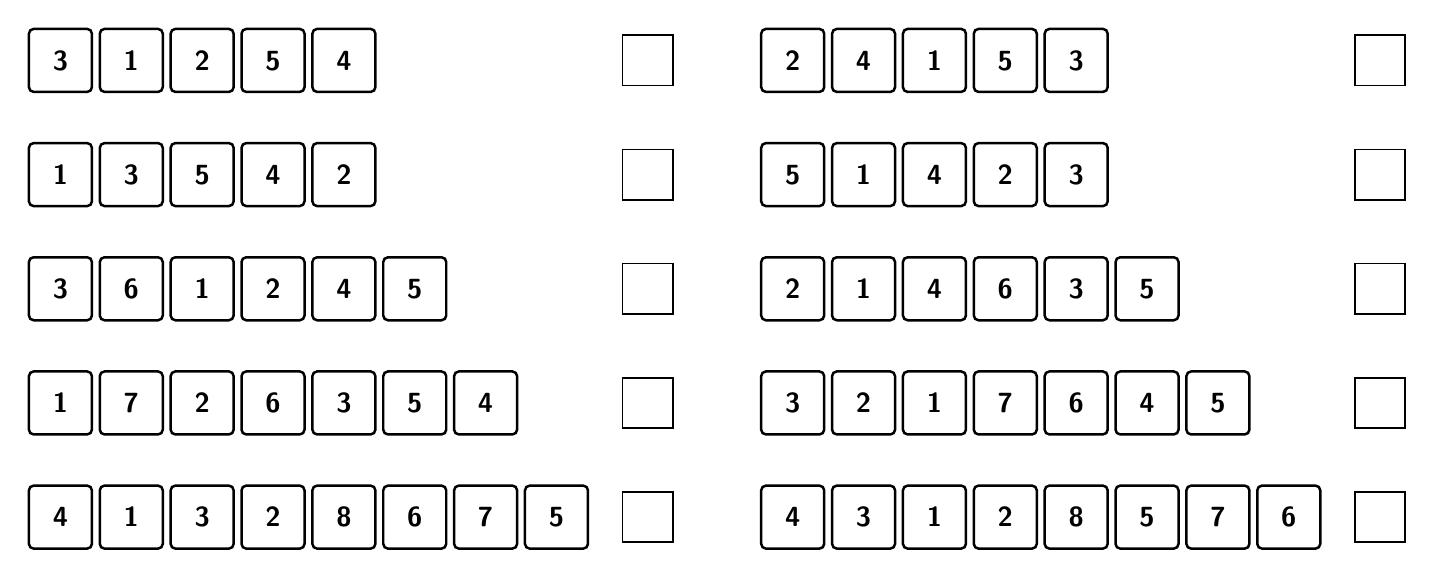
\begin{tikzpicture}[x=1mm,y=1mm]
\draw[line width=0.9pt, fill=white, rounded corners=0.6mm] (0,0) rectangle (8,8);
\node at (4,4) {\bfseries 3};
\draw[line width=0.9pt, fill=white, rounded corners=0.6mm] (9,0) rectangle (17,8);
\node at (13,4) {\bfseries 1};
\draw[line width=0.9pt, fill=white, rounded corners=0.6mm] (18,0) rectangle (26,8);
\node at (22,4) {\bfseries 2};
\draw[line width=0.9pt, fill=white, rounded corners=0.6mm] (27,0) rectangle (35,8);
\node at (31,4) {\bfseries 5};
\draw[line width=0.9pt, fill=white, rounded corners=0.6mm] (36,0) rectangle (44,8);
\node at (40,4) {\bfseries 4};
\draw[line width=0.6pt] (75.4,0.8) rectangle (81.8,7.2);
\draw[line width=0.9pt, fill=white, rounded corners=0.6mm] (93,0) rectangle (101,8);
\node at (97,4) {\bfseries 2};
\draw[line width=0.9pt, fill=white, rounded corners=0.6mm] (102,0) rectangle (110,8);
\node at (106,4) {\bfseries 4};
\draw[line width=0.9pt, fill=white, rounded corners=0.6mm] (111,0) rectangle (119,8);
\node at (115,4) {\bfseries 1};
\draw[line width=0.9pt, fill=white, rounded corners=0.6mm] (120,0) rectangle (128,8);
\node at (124,4) {\bfseries 5};
\draw[line width=0.9pt, fill=white, rounded corners=0.6mm] (129,0) rectangle (137,8);
\node at (133,4) {\bfseries 3};
\draw[line width=0.6pt] (168.4,0.8) rectangle (174.8,7.2);
\draw[line width=0.9pt, fill=white, rounded corners=0.6mm] (0,-14.5) rectangle (8,-6.5);
\node at (4,-10.5) {\bfseries 1};
\draw[line width=0.9pt, fill=white, rounded corners=0.6mm] (9,-14.5) rectangle (17,-6.5);
\node at (13,-10.5) {\bfseries 3};
\draw[line width=0.9pt, fill=white, rounded corners=0.6mm] (18,-14.5) rectangle (26,-6.5);
\node at (22,-10.5) {\bfseries 5};
\draw[line width=0.9pt, fill=white, rounded corners=0.6mm] (27,-14.5) rectangle (35,-6.5);
\node at (31,-10.5) {\bfseries 4};
\draw[line width=0.9pt, fill=white, rounded corners=0.6mm] (36,-14.5) rectangle (44,-6.5);
\node at (40,-10.5) {\bfseries 2};
\draw[line width=0.6pt] (75.4,-13.7) rectangle (81.8,-7.3);
\draw[line width=0.9pt, fill=white, rounded corners=0.6mm] (93,-14.5) rectangle (101,-6.5);
\node at (97,-10.5) {\bfseries 5};
\draw[line width=0.9pt, fill=white, rounded corners=0.6mm] (102,-14.5) rectangle (110,-6.5);
\node at (106,-10.5) {\bfseries 1};
\draw[line width=0.9pt, fill=white, rounded corners=0.6mm] (111,-14.5) rectangle (119,-6.5);
\node at (115,-10.5) {\bfseries 4};
\draw[line width=0.9pt, fill=white, rounded corners=0.6mm] (120,-14.5) rectangle (128,-6.5);
\node at (124,-10.5) {\bfseries 2};
\draw[line width=0.9pt, fill=white, rounded corners=0.6mm] (129,-14.5) rectangle (137,-6.5);
\node at (133,-10.5) {\bfseries 3};
\draw[line width=0.6pt] (168.4,-13.7) rectangle (174.8,-7.3);
\draw[line width=0.9pt, fill=white, rounded corners=0.6mm] (0,-29) rectangle (8,-21);
\node at (4,-25) {\bfseries 3};
\draw[line width=0.9pt, fill=white, rounded corners=0.6mm] (9,-29) rectangle (17,-21);
\node at (13,-25) {\bfseries 6};
\draw[line width=0.9pt, fill=white, rounded corners=0.6mm] (18,-29) rectangle (26,-21);
\node at (22,-25) {\bfseries 1};
\draw[line width=0.9pt, fill=white, rounded corners=0.6mm] (27,-29) rectangle (35,-21);
\node at (31,-25) {\bfseries 2};
\draw[line width=0.9pt, fill=white, rounded corners=0.6mm] (36,-29) rectangle (44,-21);
\node at (40,-25) {\bfseries 4};
\draw[line width=0.9pt, fill=white, rounded corners=0.6mm] (45,-29) rectangle (53,-21);
\node at (49,-25) {\bfseries 5};
\draw[line width=0.6pt] (75.4,-28.2) rectangle (81.8,-21.8);
\draw[line width=0.9pt, fill=white, rounded corners=0.6mm] (93,-29) rectangle (101,-21);
\node at (97,-25) {\bfseries 2};
\draw[line width=0.9pt, fill=white, rounded corners=0.6mm] (102,-29) rectangle (110,-21);
\node at (106,-25) {\bfseries 1};
\draw[line width=0.9pt, fill=white, rounded corners=0.6mm] (111,-29) rectangle (119,-21);
\node at (115,-25) {\bfseries 4};
\draw[line width=0.9pt, fill=white, rounded corners=0.6mm] (120,-29) rectangle (128,-21);
\node at (124,-25) {\bfseries 6};
\draw[line width=0.9pt, fill=white, rounded corners=0.6mm] (129,-29) rectangle (137,-21);
\node at (133,-25) {\bfseries 3};
\draw[line width=0.9pt, fill=white, rounded corners=0.6mm] (138,-29) rectangle (146,-21);
\node at (142,-25) {\bfseries 5};
\draw[line width=0.6pt] (168.4,-28.2) rectangle (174.8,-21.8);
\draw[line width=0.9pt, fill=white, rounded corners=0.6mm] (0,-43.5) rectangle (8,-35.5);
\node at (4,-39.5) {\bfseries 1};
\draw[line width=0.9pt, fill=white, rounded corners=0.6mm] (9,-43.5) rectangle (17,-35.5);
\node at (13,-39.5) {\bfseries 7};
\draw[line width=0.9pt, fill=white, rounded corners=0.6mm] (18,-43.5) rectangle (26,-35.5);
\node at (22,-39.5) {\bfseries 2};
\draw[line width=0.9pt, fill=white, rounded corners=0.6mm] (27,-43.5) rectangle (35,-35.5);
\node at (31,-39.5) {\bfseries 6};
\draw[line width=0.9pt, fill=white, rounded corners=0.6mm] (36,-43.5) rectangle (44,-35.5);
\node at (40,-39.5) {\bfseries 3};
\draw[line width=0.9pt, fill=white, rounded corners=0.6mm] (45,-43.5) rectangle (53,-35.5);
\node at (49,-39.5) {\bfseries 5};
\draw[line width=0.9pt, fill=white, rounded corners=0.6mm] (54,-43.5) rectangle (62,-35.5);
\node at (58,-39.5) {\bfseries 4};
\draw[line width=0.6pt] (75.4,-42.7) rectangle (81.8,-36.3);
\draw[line width=0.9pt, fill=white, rounded corners=0.6mm] (93,-43.5) rectangle (101,-35.5);
\node at (97,-39.5) {\bfseries 3};
\draw[line width=0.9pt, fill=white, rounded corners=0.6mm] (102,-43.5) rectangle (110,-35.5);
\node at (106,-39.5) {\bfseries 2};
\draw[line width=0.9pt, fill=white, rounded corners=0.6mm] (111,-43.5) rectangle (119,-35.5);
\node at (115,-39.5) {\bfseries 1};
\draw[line width=0.9pt, fill=white, rounded corners=0.6mm] (120,-43.5) rectangle (128,-35.5);
\node at (124,-39.5) {\bfseries 7};
\draw[line width=0.9pt, fill=white, rounded corners=0.6mm] (129,-43.5) rectangle (137,-35.5);
\node at (133,-39.5) {\bfseries 6};
\draw[line width=0.9pt, fill=white, rounded corners=0.6mm] (138,-43.5) rectangle (146,-35.5);
\node at (142,-39.5) {\bfseries 4};
\draw[line width=0.9pt, fill=white, rounded corners=0.6mm] (147,-43.5) rectangle (155,-35.5);
\node at (151,-39.5) {\bfseries 5};
\draw[line width=0.6pt] (168.4,-42.7) rectangle (174.8,-36.3);
\draw[line width=0.9pt, fill=white, rounded corners=0.6mm] (0,-58) rectangle (8,-50);
\node at (4,-54) {\bfseries 4};
\draw[line width=0.9pt, fill=white, rounded corners=0.6mm] (9,-58) rectangle (17,-50);
\node at (13,-54) {\bfseries 1};
\draw[line width=0.9pt, fill=white, rounded corners=0.6mm] (18,-58) rectangle (26,-50);
\node at (22,-54) {\bfseries 3};
\draw[line width=0.9pt, fill=white, rounded corners=0.6mm] (27,-58) rectangle (35,-50);
\node at (31,-54) {\bfseries 2};
\draw[line width=0.9pt, fill=white, rounded corners=0.6mm] (36,-58) rectangle (44,-50);
\node at (40,-54) {\bfseries 8};
\draw[line width=0.9pt, fill=white, rounded corners=0.6mm] (45,-58) rectangle (53,-50);
\node at (49,-54) {\bfseries 6};
\draw[line width=0.9pt, fill=white, rounded corners=0.6mm] (54,-58) rectangle (62,-50);
\node at (58,-54) {\bfseries 7};
\draw[line width=0.9pt, fill=white, rounded corners=0.6mm] (63,-58) rectangle (71,-50);
\node at (67,-54) {\bfseries 5};
\draw[line width=0.6pt] (75.4,-57.2) rectangle (81.8,-50.8);
\draw[line width=0.9pt, fill=white, rounded corners=0.6mm] (93,-58) rectangle (101,-50);
\node at (97,-54) {\bfseries 4};
\draw[line width=0.9pt, fill=white, rounded corners=0.6mm] (102,-58) rectangle (110,-50);
\node at (106,-54) {\bfseries 3};
\draw[line width=0.9pt, fill=white, rounded corners=0.6mm] (111,-58) rectangle (119,-50);
\node at (115,-54) {\bfseries 1};
\draw[line width=0.9pt, fill=white, rounded corners=0.6mm] (120,-58) rectangle (128,-50);
\node at (124,-54) {\bfseries 2};
\draw[line width=0.9pt, fill=white, rounded corners=0.6mm] (129,-58) rectangle (137,-50);
\node at (133,-54) {\bfseries 8};
\draw[line width=0.9pt, fill=white, rounded corners=0.6mm] (138,-58) rectangle (146,-50);
\node at (142,-54) {\bfseries 5};
\draw[line width=0.9pt, fill=white, rounded corners=0.6mm] (147,-58) rectangle (155,-50);
\node at (151,-54) {\bfseries 7};
\draw[line width=0.9pt, fill=white, rounded corners=0.6mm] (156,-58) rectangle (164,-50);
\node at (160,-54) {\bfseries 6};
\draw[line width=0.6pt] (168.4,-57.2) rectangle (174.8,-50.8);
\end{tikzpicture}
\end{center}

\vspace{4pt}
\problem{3}Find a way to tell from its numbers alone whether a train can leave in order. Explain why your way always gives the right answer.
\par\vspace{3pt}\noindent\begin{tikzpicture}[x=1mm,y=1mm]
\draw[black!30, line width=0.4pt] (0,-9) -- (177,-9);
\draw[black!30, line width=0.4pt] (0,-18) -- (177,-18);
\draw[black!30, line width=0.4pt] (0,-27) -- (177,-27);
\draw[black!30, line width=0.4pt] (0,-36) -- (177,-36);
\draw[black!30, line width=0.4pt] (0,-45) -- (177,-45);
\draw[black!30, line width=0.4pt] (0,-54) -- (177,-54);
\draw[black!30, line width=0.4pt] (0,-63) -- (177,-63);
\draw[black!30, line width=0.4pt] (0,-72) -- (177,-72);
\draw[black!30, line width=0.4pt] (0,-81) -- (177,-81);
\draw[black!30, line width=0.4pt] (0,-90) -- (177,-90);
\end{tikzpicture}\par
\newpage
\problem{4}A drive can be recorded as a path that steps up when a car goes into the siding and steps down when a car comes out, as shown for the train 1 3 2. Draw a path for each four-car train that can leave in order, and write the train under its path.
\par\vspace{4pt}\begin{center}
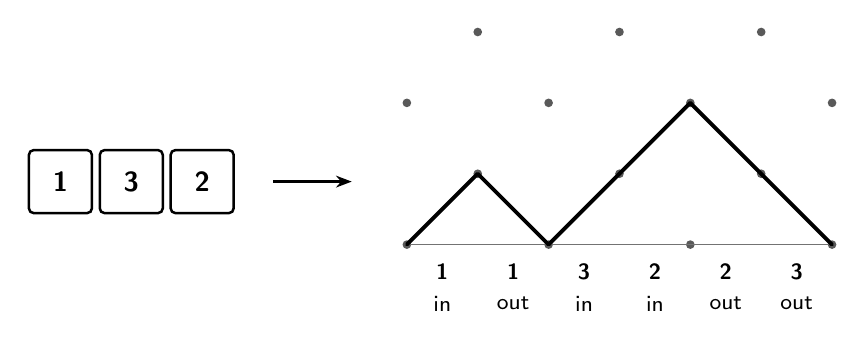
\begin{tikzpicture}[x=1mm,y=1mm]
\draw[line width=0.9pt, fill=white, rounded corners=0.6mm] (0,4) rectangle (8,12);
\node at (4,8) {\bfseries 1};
\draw[line width=0.9pt, fill=white, rounded corners=0.6mm] (9,4) rectangle (17,12);
\node at (13,8) {\bfseries 3};
\draw[line width=0.9pt, fill=white, rounded corners=0.6mm] (18,4) rectangle (26,12);
\node at (22,8) {\bfseries 2};
\draw[-{Stealth[length=2mm]}, line width=0.9pt] (31,8) -- (41,8);
\fill[black!65] (48,0) circle (0.55);
\fill[black!65] (48,18) circle (0.55);
\fill[black!65] (57,9) circle (0.55);
\fill[black!65] (57,27) circle (0.55);
\fill[black!65] (66,0) circle (0.55);
\fill[black!65] (66,18) circle (0.55);
\fill[black!65] (75,9) circle (0.55);
\fill[black!65] (75,27) circle (0.55);
\fill[black!65] (84,0) circle (0.55);
\fill[black!65] (84,18) circle (0.55);
\fill[black!65] (93,9) circle (0.55);
\fill[black!65] (93,27) circle (0.55);
\fill[black!65] (102,0) circle (0.55);
\fill[black!65] (102,18) circle (0.55);
\draw[black!55, line width=0.6pt] (48,0) -- (102,0);
\draw[line width=1.4pt, line join=round, line cap=round] (48,0) -- (57,9) -- (66,0) -- (75,9) -- (84,18) -- (93,9) -- (102,0);
\node[font=\footnotesize\bfseries] at (52.5,-3.5) {1};
\node[font=\footnotesize] at (52.5,-7.5) {in};
\node[font=\footnotesize\bfseries] at (61.5,-3.5) {1};
\node[font=\footnotesize] at (61.5,-7.5) {out};
\node[font=\footnotesize\bfseries] at (70.5,-3.5) {3};
\node[font=\footnotesize] at (70.5,-7.5) {in};
\node[font=\footnotesize\bfseries] at (79.5,-3.5) {2};
\node[font=\footnotesize] at (79.5,-7.5) {in};
\node[font=\footnotesize\bfseries] at (88.5,-3.5) {2};
\node[font=\footnotesize] at (88.5,-7.5) {out};
\node[font=\footnotesize\bfseries] at (97.5,-3.5) {3};
\node[font=\footnotesize] at (97.5,-7.5) {out};
\end{tikzpicture}
\end{center}

\par\vspace{6pt}\begin{center}
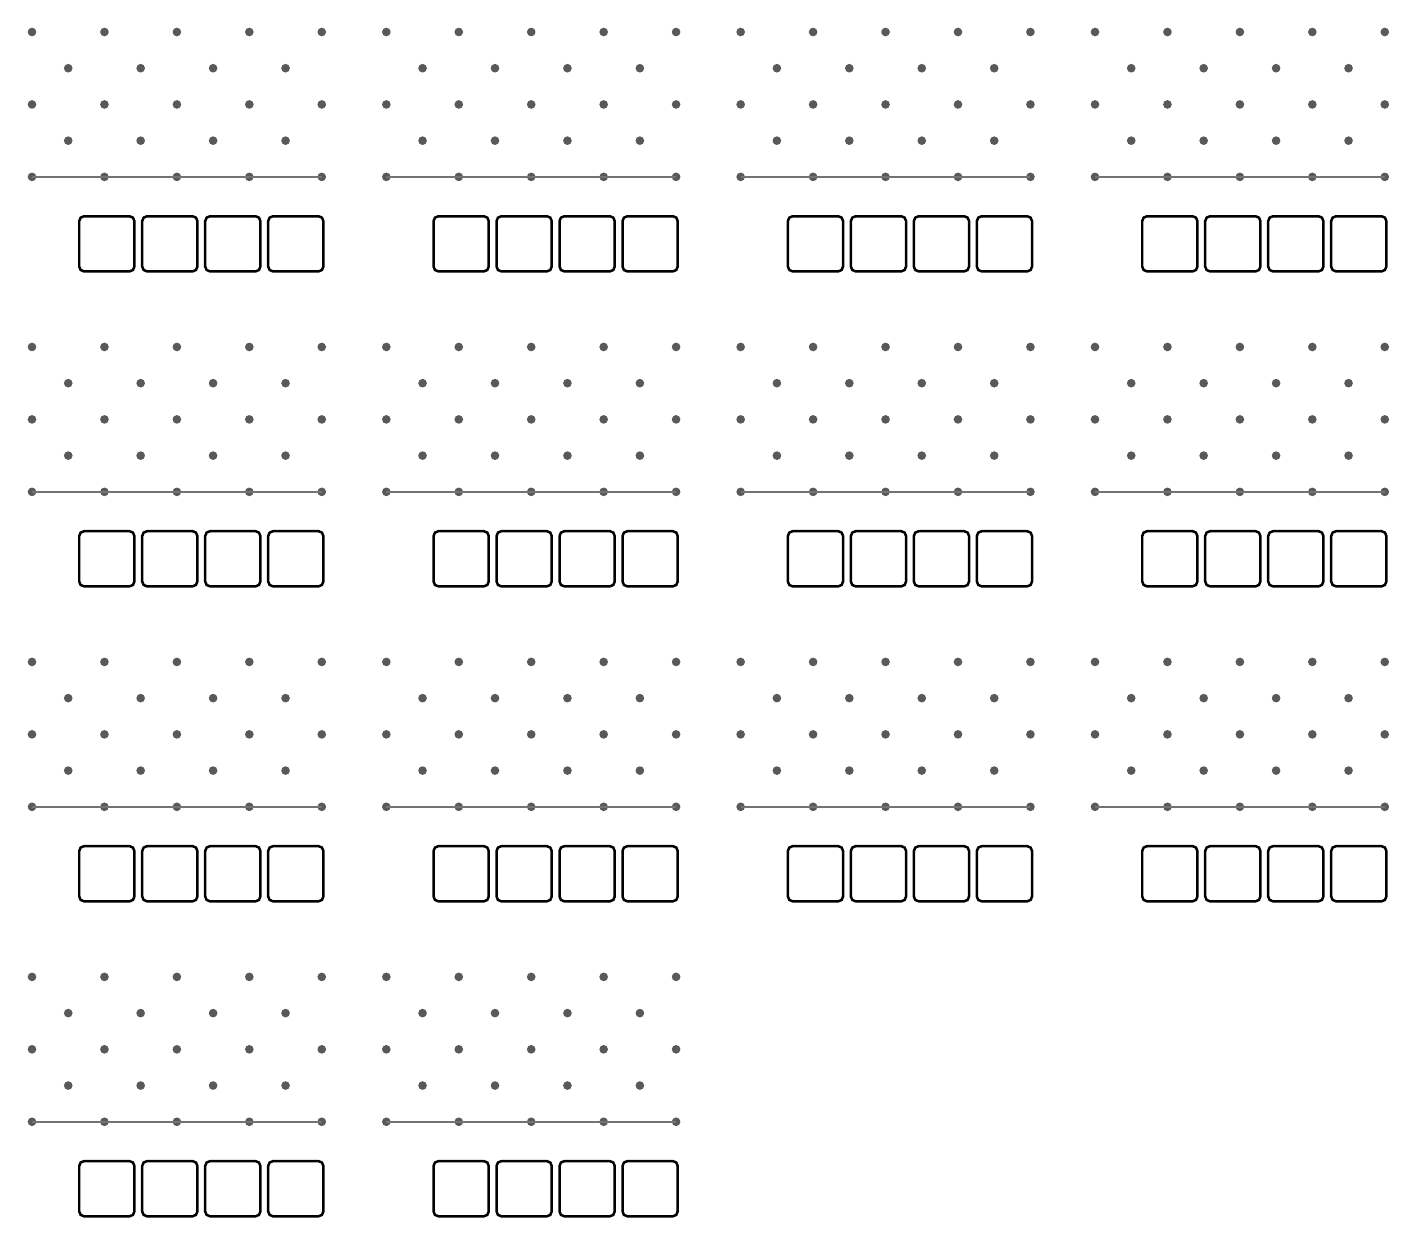
\begin{tikzpicture}[x=1mm,y=1mm]
\fill[black!65] (0,0) circle (0.55);
\fill[black!65] (0,9.2) circle (0.55);
\fill[black!65] (0,18.4) circle (0.55);
\fill[black!65] (4.6,4.6) circle (0.55);
\fill[black!65] (4.6,13.8) circle (0.55);
\fill[black!65] (9.2,0) circle (0.55);
\fill[black!65] (9.2,9.2) circle (0.55);
\fill[black!65] (9.2,18.4) circle (0.55);
\fill[black!65] (13.8,4.6) circle (0.55);
\fill[black!65] (13.8,13.8) circle (0.55);
\fill[black!65] (18.4,0) circle (0.55);
\fill[black!65] (18.4,9.2) circle (0.55);
\fill[black!65] (18.4,18.4) circle (0.55);
\fill[black!65] (23,4.6) circle (0.55);
\fill[black!65] (23,13.8) circle (0.55);
\fill[black!65] (27.6,0) circle (0.55);
\fill[black!65] (27.6,9.2) circle (0.55);
\fill[black!65] (27.6,18.4) circle (0.55);
\fill[black!65] (32.2,4.6) circle (0.55);
\fill[black!65] (32.2,13.8) circle (0.55);
\fill[black!65] (36.8,0) circle (0.55);
\fill[black!65] (36.8,9.2) circle (0.55);
\fill[black!65] (36.8,18.4) circle (0.55);
\draw[black!55, line width=0.6pt] (0,0) -- (36.8,0);
\draw[line width=0.9pt, fill=white, rounded corners=0.6mm] (6,-12) rectangle (13,-5);
\draw[line width=0.9pt, fill=white, rounded corners=0.6mm] (14,-12) rectangle (21,-5);
\draw[line width=0.9pt, fill=white, rounded corners=0.6mm] (22,-12) rectangle (29,-5);
\draw[line width=0.9pt, fill=white, rounded corners=0.6mm] (30,-12) rectangle (37,-5);
\fill[black!65] (45,0) circle (0.55);
\fill[black!65] (45,9.2) circle (0.55);
\fill[black!65] (45,18.4) circle (0.55);
\fill[black!65] (49.6,4.6) circle (0.55);
\fill[black!65] (49.6,13.8) circle (0.55);
\fill[black!65] (54.2,0) circle (0.55);
\fill[black!65] (54.2,9.2) circle (0.55);
\fill[black!65] (54.2,18.4) circle (0.55);
\fill[black!65] (58.8,4.6) circle (0.55);
\fill[black!65] (58.8,13.8) circle (0.55);
\fill[black!65] (63.4,0) circle (0.55);
\fill[black!65] (63.4,9.2) circle (0.55);
\fill[black!65] (63.4,18.4) circle (0.55);
\fill[black!65] (68,4.6) circle (0.55);
\fill[black!65] (68,13.8) circle (0.55);
\fill[black!65] (72.6,0) circle (0.55);
\fill[black!65] (72.6,9.2) circle (0.55);
\fill[black!65] (72.6,18.4) circle (0.55);
\fill[black!65] (77.2,4.6) circle (0.55);
\fill[black!65] (77.2,13.8) circle (0.55);
\fill[black!65] (81.8,0) circle (0.55);
\fill[black!65] (81.8,9.2) circle (0.55);
\fill[black!65] (81.8,18.4) circle (0.55);
\draw[black!55, line width=0.6pt] (45,0) -- (81.8,0);
\draw[line width=0.9pt, fill=white, rounded corners=0.6mm] (51,-12) rectangle (58,-5);
\draw[line width=0.9pt, fill=white, rounded corners=0.6mm] (59,-12) rectangle (66,-5);
\draw[line width=0.9pt, fill=white, rounded corners=0.6mm] (67,-12) rectangle (74,-5);
\draw[line width=0.9pt, fill=white, rounded corners=0.6mm] (75,-12) rectangle (82,-5);
\fill[black!65] (90,0) circle (0.55);
\fill[black!65] (90,9.2) circle (0.55);
\fill[black!65] (90,18.4) circle (0.55);
\fill[black!65] (94.6,4.6) circle (0.55);
\fill[black!65] (94.6,13.8) circle (0.55);
\fill[black!65] (99.2,0) circle (0.55);
\fill[black!65] (99.2,9.2) circle (0.55);
\fill[black!65] (99.2,18.4) circle (0.55);
\fill[black!65] (103.8,4.6) circle (0.55);
\fill[black!65] (103.8,13.8) circle (0.55);
\fill[black!65] (108.4,0) circle (0.55);
\fill[black!65] (108.4,9.2) circle (0.55);
\fill[black!65] (108.4,18.4) circle (0.55);
\fill[black!65] (113,4.6) circle (0.55);
\fill[black!65] (113,13.8) circle (0.55);
\fill[black!65] (117.6,0) circle (0.55);
\fill[black!65] (117.6,9.2) circle (0.55);
\fill[black!65] (117.6,18.4) circle (0.55);
\fill[black!65] (122.2,4.6) circle (0.55);
\fill[black!65] (122.2,13.8) circle (0.55);
\fill[black!65] (126.8,0) circle (0.55);
\fill[black!65] (126.8,9.2) circle (0.55);
\fill[black!65] (126.8,18.4) circle (0.55);
\draw[black!55, line width=0.6pt] (90,0) -- (126.8,0);
\draw[line width=0.9pt, fill=white, rounded corners=0.6mm] (96,-12) rectangle (103,-5);
\draw[line width=0.9pt, fill=white, rounded corners=0.6mm] (104,-12) rectangle (111,-5);
\draw[line width=0.9pt, fill=white, rounded corners=0.6mm] (112,-12) rectangle (119,-5);
\draw[line width=0.9pt, fill=white, rounded corners=0.6mm] (120,-12) rectangle (127,-5);
\fill[black!65] (135,0) circle (0.55);
\fill[black!65] (135,9.2) circle (0.55);
\fill[black!65] (135,18.4) circle (0.55);
\fill[black!65] (139.6,4.6) circle (0.55);
\fill[black!65] (139.6,13.8) circle (0.55);
\fill[black!65] (144.2,0) circle (0.55);
\fill[black!65] (144.2,9.2) circle (0.55);
\fill[black!65] (144.2,18.4) circle (0.55);
\fill[black!65] (148.8,4.6) circle (0.55);
\fill[black!65] (148.8,13.8) circle (0.55);
\fill[black!65] (153.4,0) circle (0.55);
\fill[black!65] (153.4,9.2) circle (0.55);
\fill[black!65] (153.4,18.4) circle (0.55);
\fill[black!65] (158,4.6) circle (0.55);
\fill[black!65] (158,13.8) circle (0.55);
\fill[black!65] (162.6,0) circle (0.55);
\fill[black!65] (162.6,9.2) circle (0.55);
\fill[black!65] (162.6,18.4) circle (0.55);
\fill[black!65] (167.2,4.6) circle (0.55);
\fill[black!65] (167.2,13.8) circle (0.55);
\fill[black!65] (171.8,0) circle (0.55);
\fill[black!65] (171.8,9.2) circle (0.55);
\fill[black!65] (171.8,18.4) circle (0.55);
\draw[black!55, line width=0.6pt] (135,0) -- (171.8,0);
\draw[line width=0.9pt, fill=white, rounded corners=0.6mm] (141,-12) rectangle (148,-5);
\draw[line width=0.9pt, fill=white, rounded corners=0.6mm] (149,-12) rectangle (156,-5);
\draw[line width=0.9pt, fill=white, rounded corners=0.6mm] (157,-12) rectangle (164,-5);
\draw[line width=0.9pt, fill=white, rounded corners=0.6mm] (165,-12) rectangle (172,-5);
\fill[black!65] (0,-40) circle (0.55);
\fill[black!65] (0,-30.8) circle (0.55);
\fill[black!65] (0,-21.6) circle (0.55);
\fill[black!65] (4.6,-35.4) circle (0.55);
\fill[black!65] (4.6,-26.2) circle (0.55);
\fill[black!65] (9.2,-40) circle (0.55);
\fill[black!65] (9.2,-30.8) circle (0.55);
\fill[black!65] (9.2,-21.6) circle (0.55);
\fill[black!65] (13.8,-35.4) circle (0.55);
\fill[black!65] (13.8,-26.2) circle (0.55);
\fill[black!65] (18.4,-40) circle (0.55);
\fill[black!65] (18.4,-30.8) circle (0.55);
\fill[black!65] (18.4,-21.6) circle (0.55);
\fill[black!65] (23,-35.4) circle (0.55);
\fill[black!65] (23,-26.2) circle (0.55);
\fill[black!65] (27.6,-40) circle (0.55);
\fill[black!65] (27.6,-30.8) circle (0.55);
\fill[black!65] (27.6,-21.6) circle (0.55);
\fill[black!65] (32.2,-35.4) circle (0.55);
\fill[black!65] (32.2,-26.2) circle (0.55);
\fill[black!65] (36.8,-40) circle (0.55);
\fill[black!65] (36.8,-30.8) circle (0.55);
\fill[black!65] (36.8,-21.6) circle (0.55);
\draw[black!55, line width=0.6pt] (0,-40) -- (36.8,-40);
\draw[line width=0.9pt, fill=white, rounded corners=0.6mm] (6,-52) rectangle (13,-45);
\draw[line width=0.9pt, fill=white, rounded corners=0.6mm] (14,-52) rectangle (21,-45);
\draw[line width=0.9pt, fill=white, rounded corners=0.6mm] (22,-52) rectangle (29,-45);
\draw[line width=0.9pt, fill=white, rounded corners=0.6mm] (30,-52) rectangle (37,-45);
\fill[black!65] (45,-40) circle (0.55);
\fill[black!65] (45,-30.8) circle (0.55);
\fill[black!65] (45,-21.6) circle (0.55);
\fill[black!65] (49.6,-35.4) circle (0.55);
\fill[black!65] (49.6,-26.2) circle (0.55);
\fill[black!65] (54.2,-40) circle (0.55);
\fill[black!65] (54.2,-30.8) circle (0.55);
\fill[black!65] (54.2,-21.6) circle (0.55);
\fill[black!65] (58.8,-35.4) circle (0.55);
\fill[black!65] (58.8,-26.2) circle (0.55);
\fill[black!65] (63.4,-40) circle (0.55);
\fill[black!65] (63.4,-30.8) circle (0.55);
\fill[black!65] (63.4,-21.6) circle (0.55);
\fill[black!65] (68,-35.4) circle (0.55);
\fill[black!65] (68,-26.2) circle (0.55);
\fill[black!65] (72.6,-40) circle (0.55);
\fill[black!65] (72.6,-30.8) circle (0.55);
\fill[black!65] (72.6,-21.6) circle (0.55);
\fill[black!65] (77.2,-35.4) circle (0.55);
\fill[black!65] (77.2,-26.2) circle (0.55);
\fill[black!65] (81.8,-40) circle (0.55);
\fill[black!65] (81.8,-30.8) circle (0.55);
\fill[black!65] (81.8,-21.6) circle (0.55);
\draw[black!55, line width=0.6pt] (45,-40) -- (81.8,-40);
\draw[line width=0.9pt, fill=white, rounded corners=0.6mm] (51,-52) rectangle (58,-45);
\draw[line width=0.9pt, fill=white, rounded corners=0.6mm] (59,-52) rectangle (66,-45);
\draw[line width=0.9pt, fill=white, rounded corners=0.6mm] (67,-52) rectangle (74,-45);
\draw[line width=0.9pt, fill=white, rounded corners=0.6mm] (75,-52) rectangle (82,-45);
\fill[black!65] (90,-40) circle (0.55);
\fill[black!65] (90,-30.8) circle (0.55);
\fill[black!65] (90,-21.6) circle (0.55);
\fill[black!65] (94.6,-35.4) circle (0.55);
\fill[black!65] (94.6,-26.2) circle (0.55);
\fill[black!65] (99.2,-40) circle (0.55);
\fill[black!65] (99.2,-30.8) circle (0.55);
\fill[black!65] (99.2,-21.6) circle (0.55);
\fill[black!65] (103.8,-35.4) circle (0.55);
\fill[black!65] (103.8,-26.2) circle (0.55);
\fill[black!65] (108.4,-40) circle (0.55);
\fill[black!65] (108.4,-30.8) circle (0.55);
\fill[black!65] (108.4,-21.6) circle (0.55);
\fill[black!65] (113,-35.4) circle (0.55);
\fill[black!65] (113,-26.2) circle (0.55);
\fill[black!65] (117.6,-40) circle (0.55);
\fill[black!65] (117.6,-30.8) circle (0.55);
\fill[black!65] (117.6,-21.6) circle (0.55);
\fill[black!65] (122.2,-35.4) circle (0.55);
\fill[black!65] (122.2,-26.2) circle (0.55);
\fill[black!65] (126.8,-40) circle (0.55);
\fill[black!65] (126.8,-30.8) circle (0.55);
\fill[black!65] (126.8,-21.6) circle (0.55);
\draw[black!55, line width=0.6pt] (90,-40) -- (126.8,-40);
\draw[line width=0.9pt, fill=white, rounded corners=0.6mm] (96,-52) rectangle (103,-45);
\draw[line width=0.9pt, fill=white, rounded corners=0.6mm] (104,-52) rectangle (111,-45);
\draw[line width=0.9pt, fill=white, rounded corners=0.6mm] (112,-52) rectangle (119,-45);
\draw[line width=0.9pt, fill=white, rounded corners=0.6mm] (120,-52) rectangle (127,-45);
\fill[black!65] (135,-40) circle (0.55);
\fill[black!65] (135,-30.8) circle (0.55);
\fill[black!65] (135,-21.6) circle (0.55);
\fill[black!65] (139.6,-35.4) circle (0.55);
\fill[black!65] (139.6,-26.2) circle (0.55);
\fill[black!65] (144.2,-40) circle (0.55);
\fill[black!65] (144.2,-30.8) circle (0.55);
\fill[black!65] (144.2,-21.6) circle (0.55);
\fill[black!65] (148.8,-35.4) circle (0.55);
\fill[black!65] (148.8,-26.2) circle (0.55);
\fill[black!65] (153.4,-40) circle (0.55);
\fill[black!65] (153.4,-30.8) circle (0.55);
\fill[black!65] (153.4,-21.6) circle (0.55);
\fill[black!65] (158,-35.4) circle (0.55);
\fill[black!65] (158,-26.2) circle (0.55);
\fill[black!65] (162.6,-40) circle (0.55);
\fill[black!65] (162.6,-30.8) circle (0.55);
\fill[black!65] (162.6,-21.6) circle (0.55);
\fill[black!65] (167.2,-35.4) circle (0.55);
\fill[black!65] (167.2,-26.2) circle (0.55);
\fill[black!65] (171.8,-40) circle (0.55);
\fill[black!65] (171.8,-30.8) circle (0.55);
\fill[black!65] (171.8,-21.6) circle (0.55);
\draw[black!55, line width=0.6pt] (135,-40) -- (171.8,-40);
\draw[line width=0.9pt, fill=white, rounded corners=0.6mm] (141,-52) rectangle (148,-45);
\draw[line width=0.9pt, fill=white, rounded corners=0.6mm] (149,-52) rectangle (156,-45);
\draw[line width=0.9pt, fill=white, rounded corners=0.6mm] (157,-52) rectangle (164,-45);
\draw[line width=0.9pt, fill=white, rounded corners=0.6mm] (165,-52) rectangle (172,-45);
\fill[black!65] (0,-80) circle (0.55);
\fill[black!65] (0,-70.8) circle (0.55);
\fill[black!65] (0,-61.6) circle (0.55);
\fill[black!65] (4.6,-75.4) circle (0.55);
\fill[black!65] (4.6,-66.2) circle (0.55);
\fill[black!65] (9.2,-80) circle (0.55);
\fill[black!65] (9.2,-70.8) circle (0.55);
\fill[black!65] (9.2,-61.6) circle (0.55);
\fill[black!65] (13.8,-75.4) circle (0.55);
\fill[black!65] (13.8,-66.2) circle (0.55);
\fill[black!65] (18.4,-80) circle (0.55);
\fill[black!65] (18.4,-70.8) circle (0.55);
\fill[black!65] (18.4,-61.6) circle (0.55);
\fill[black!65] (23,-75.4) circle (0.55);
\fill[black!65] (23,-66.2) circle (0.55);
\fill[black!65] (27.6,-80) circle (0.55);
\fill[black!65] (27.6,-70.8) circle (0.55);
\fill[black!65] (27.6,-61.6) circle (0.55);
\fill[black!65] (32.2,-75.4) circle (0.55);
\fill[black!65] (32.2,-66.2) circle (0.55);
\fill[black!65] (36.8,-80) circle (0.55);
\fill[black!65] (36.8,-70.8) circle (0.55);
\fill[black!65] (36.8,-61.6) circle (0.55);
\draw[black!55, line width=0.6pt] (0,-80) -- (36.8,-80);
\draw[line width=0.9pt, fill=white, rounded corners=0.6mm] (6,-92) rectangle (13,-85);
\draw[line width=0.9pt, fill=white, rounded corners=0.6mm] (14,-92) rectangle (21,-85);
\draw[line width=0.9pt, fill=white, rounded corners=0.6mm] (22,-92) rectangle (29,-85);
\draw[line width=0.9pt, fill=white, rounded corners=0.6mm] (30,-92) rectangle (37,-85);
\fill[black!65] (45,-80) circle (0.55);
\fill[black!65] (45,-70.8) circle (0.55);
\fill[black!65] (45,-61.6) circle (0.55);
\fill[black!65] (49.6,-75.4) circle (0.55);
\fill[black!65] (49.6,-66.2) circle (0.55);
\fill[black!65] (54.2,-80) circle (0.55);
\fill[black!65] (54.2,-70.8) circle (0.55);
\fill[black!65] (54.2,-61.6) circle (0.55);
\fill[black!65] (58.8,-75.4) circle (0.55);
\fill[black!65] (58.8,-66.2) circle (0.55);
\fill[black!65] (63.4,-80) circle (0.55);
\fill[black!65] (63.4,-70.8) circle (0.55);
\fill[black!65] (63.4,-61.6) circle (0.55);
\fill[black!65] (68,-75.4) circle (0.55);
\fill[black!65] (68,-66.2) circle (0.55);
\fill[black!65] (72.6,-80) circle (0.55);
\fill[black!65] (72.6,-70.8) circle (0.55);
\fill[black!65] (72.6,-61.6) circle (0.55);
\fill[black!65] (77.2,-75.4) circle (0.55);
\fill[black!65] (77.2,-66.2) circle (0.55);
\fill[black!65] (81.8,-80) circle (0.55);
\fill[black!65] (81.8,-70.8) circle (0.55);
\fill[black!65] (81.8,-61.6) circle (0.55);
\draw[black!55, line width=0.6pt] (45,-80) -- (81.8,-80);
\draw[line width=0.9pt, fill=white, rounded corners=0.6mm] (51,-92) rectangle (58,-85);
\draw[line width=0.9pt, fill=white, rounded corners=0.6mm] (59,-92) rectangle (66,-85);
\draw[line width=0.9pt, fill=white, rounded corners=0.6mm] (67,-92) rectangle (74,-85);
\draw[line width=0.9pt, fill=white, rounded corners=0.6mm] (75,-92) rectangle (82,-85);
\fill[black!65] (90,-80) circle (0.55);
\fill[black!65] (90,-70.8) circle (0.55);
\fill[black!65] (90,-61.6) circle (0.55);
\fill[black!65] (94.6,-75.4) circle (0.55);
\fill[black!65] (94.6,-66.2) circle (0.55);
\fill[black!65] (99.2,-80) circle (0.55);
\fill[black!65] (99.2,-70.8) circle (0.55);
\fill[black!65] (99.2,-61.6) circle (0.55);
\fill[black!65] (103.8,-75.4) circle (0.55);
\fill[black!65] (103.8,-66.2) circle (0.55);
\fill[black!65] (108.4,-80) circle (0.55);
\fill[black!65] (108.4,-70.8) circle (0.55);
\fill[black!65] (108.4,-61.6) circle (0.55);
\fill[black!65] (113,-75.4) circle (0.55);
\fill[black!65] (113,-66.2) circle (0.55);
\fill[black!65] (117.6,-80) circle (0.55);
\fill[black!65] (117.6,-70.8) circle (0.55);
\fill[black!65] (117.6,-61.6) circle (0.55);
\fill[black!65] (122.2,-75.4) circle (0.55);
\fill[black!65] (122.2,-66.2) circle (0.55);
\fill[black!65] (126.8,-80) circle (0.55);
\fill[black!65] (126.8,-70.8) circle (0.55);
\fill[black!65] (126.8,-61.6) circle (0.55);
\draw[black!55, line width=0.6pt] (90,-80) -- (126.8,-80);
\draw[line width=0.9pt, fill=white, rounded corners=0.6mm] (96,-92) rectangle (103,-85);
\draw[line width=0.9pt, fill=white, rounded corners=0.6mm] (104,-92) rectangle (111,-85);
\draw[line width=0.9pt, fill=white, rounded corners=0.6mm] (112,-92) rectangle (119,-85);
\draw[line width=0.9pt, fill=white, rounded corners=0.6mm] (120,-92) rectangle (127,-85);
\fill[black!65] (135,-80) circle (0.55);
\fill[black!65] (135,-70.8) circle (0.55);
\fill[black!65] (135,-61.6) circle (0.55);
\fill[black!65] (139.6,-75.4) circle (0.55);
\fill[black!65] (139.6,-66.2) circle (0.55);
\fill[black!65] (144.2,-80) circle (0.55);
\fill[black!65] (144.2,-70.8) circle (0.55);
\fill[black!65] (144.2,-61.6) circle (0.55);
\fill[black!65] (148.8,-75.4) circle (0.55);
\fill[black!65] (148.8,-66.2) circle (0.55);
\fill[black!65] (153.4,-80) circle (0.55);
\fill[black!65] (153.4,-70.8) circle (0.55);
\fill[black!65] (153.4,-61.6) circle (0.55);
\fill[black!65] (158,-75.4) circle (0.55);
\fill[black!65] (158,-66.2) circle (0.55);
\fill[black!65] (162.6,-80) circle (0.55);
\fill[black!65] (162.6,-70.8) circle (0.55);
\fill[black!65] (162.6,-61.6) circle (0.55);
\fill[black!65] (167.2,-75.4) circle (0.55);
\fill[black!65] (167.2,-66.2) circle (0.55);
\fill[black!65] (171.8,-80) circle (0.55);
\fill[black!65] (171.8,-70.8) circle (0.55);
\fill[black!65] (171.8,-61.6) circle (0.55);
\draw[black!55, line width=0.6pt] (135,-80) -- (171.8,-80);
\draw[line width=0.9pt, fill=white, rounded corners=0.6mm] (141,-92) rectangle (148,-85);
\draw[line width=0.9pt, fill=white, rounded corners=0.6mm] (149,-92) rectangle (156,-85);
\draw[line width=0.9pt, fill=white, rounded corners=0.6mm] (157,-92) rectangle (164,-85);
\draw[line width=0.9pt, fill=white, rounded corners=0.6mm] (165,-92) rectangle (172,-85);
\fill[black!65] (0,-120) circle (0.55);
\fill[black!65] (0,-110.8) circle (0.55);
\fill[black!65] (0,-101.6) circle (0.55);
\fill[black!65] (4.6,-115.4) circle (0.55);
\fill[black!65] (4.6,-106.2) circle (0.55);
\fill[black!65] (9.2,-120) circle (0.55);
\fill[black!65] (9.2,-110.8) circle (0.55);
\fill[black!65] (9.2,-101.6) circle (0.55);
\fill[black!65] (13.8,-115.4) circle (0.55);
\fill[black!65] (13.8,-106.2) circle (0.55);
\fill[black!65] (18.4,-120) circle (0.55);
\fill[black!65] (18.4,-110.8) circle (0.55);
\fill[black!65] (18.4,-101.6) circle (0.55);
\fill[black!65] (23,-115.4) circle (0.55);
\fill[black!65] (23,-106.2) circle (0.55);
\fill[black!65] (27.6,-120) circle (0.55);
\fill[black!65] (27.6,-110.8) circle (0.55);
\fill[black!65] (27.6,-101.6) circle (0.55);
\fill[black!65] (32.2,-115.4) circle (0.55);
\fill[black!65] (32.2,-106.2) circle (0.55);
\fill[black!65] (36.8,-120) circle (0.55);
\fill[black!65] (36.8,-110.8) circle (0.55);
\fill[black!65] (36.8,-101.6) circle (0.55);
\draw[black!55, line width=0.6pt] (0,-120) -- (36.8,-120);
\draw[line width=0.9pt, fill=white, rounded corners=0.6mm] (6,-132) rectangle (13,-125);
\draw[line width=0.9pt, fill=white, rounded corners=0.6mm] (14,-132) rectangle (21,-125);
\draw[line width=0.9pt, fill=white, rounded corners=0.6mm] (22,-132) rectangle (29,-125);
\draw[line width=0.9pt, fill=white, rounded corners=0.6mm] (30,-132) rectangle (37,-125);
\fill[black!65] (45,-120) circle (0.55);
\fill[black!65] (45,-110.8) circle (0.55);
\fill[black!65] (45,-101.6) circle (0.55);
\fill[black!65] (49.6,-115.4) circle (0.55);
\fill[black!65] (49.6,-106.2) circle (0.55);
\fill[black!65] (54.2,-120) circle (0.55);
\fill[black!65] (54.2,-110.8) circle (0.55);
\fill[black!65] (54.2,-101.6) circle (0.55);
\fill[black!65] (58.8,-115.4) circle (0.55);
\fill[black!65] (58.8,-106.2) circle (0.55);
\fill[black!65] (63.4,-120) circle (0.55);
\fill[black!65] (63.4,-110.8) circle (0.55);
\fill[black!65] (63.4,-101.6) circle (0.55);
\fill[black!65] (68,-115.4) circle (0.55);
\fill[black!65] (68,-106.2) circle (0.55);
\fill[black!65] (72.6,-120) circle (0.55);
\fill[black!65] (72.6,-110.8) circle (0.55);
\fill[black!65] (72.6,-101.6) circle (0.55);
\fill[black!65] (77.2,-115.4) circle (0.55);
\fill[black!65] (77.2,-106.2) circle (0.55);
\fill[black!65] (81.8,-120) circle (0.55);
\fill[black!65] (81.8,-110.8) circle (0.55);
\fill[black!65] (81.8,-101.6) circle (0.55);
\draw[black!55, line width=0.6pt] (45,-120) -- (81.8,-120);
\draw[line width=0.9pt, fill=white, rounded corners=0.6mm] (51,-132) rectangle (58,-125);
\draw[line width=0.9pt, fill=white, rounded corners=0.6mm] (59,-132) rectangle (66,-125);
\draw[line width=0.9pt, fill=white, rounded corners=0.6mm] (67,-132) rectangle (74,-125);
\draw[line width=0.9pt, fill=white, rounded corners=0.6mm] (75,-132) rectangle (82,-125);
\end{tikzpicture}
\end{center}

\newpage
\problem{5}Each of these paths comes from a five-car train that leaves in order. Find the train for each path.
\par\vspace{8pt}\begin{center}
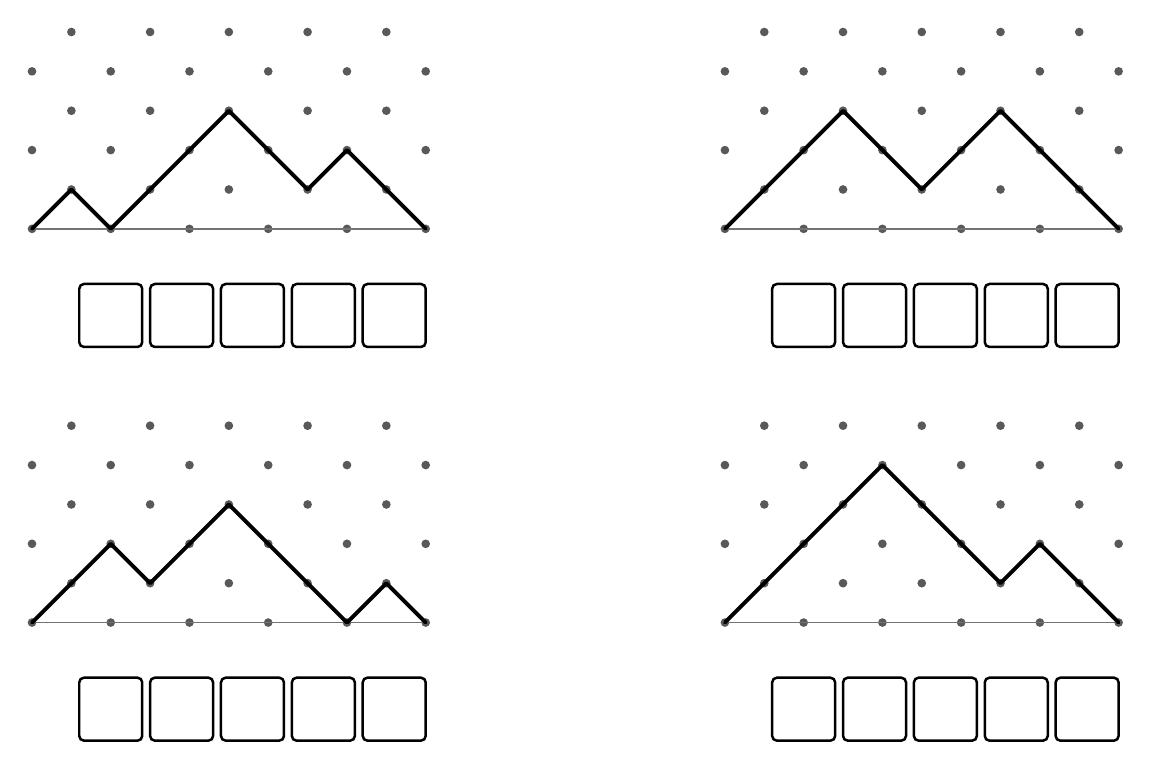
\begin{tikzpicture}[x=1mm,y=1mm]
\fill[black!65] (0,0) circle (0.55);
\fill[black!65] (0,10) circle (0.55);
\fill[black!65] (0,20) circle (0.55);
\fill[black!65] (5,5) circle (0.55);
\fill[black!65] (5,15) circle (0.55);
\fill[black!65] (5,25) circle (0.55);
\fill[black!65] (10,0) circle (0.55);
\fill[black!65] (10,10) circle (0.55);
\fill[black!65] (10,20) circle (0.55);
\fill[black!65] (15,5) circle (0.55);
\fill[black!65] (15,15) circle (0.55);
\fill[black!65] (15,25) circle (0.55);
\fill[black!65] (20,0) circle (0.55);
\fill[black!65] (20,10) circle (0.55);
\fill[black!65] (20,20) circle (0.55);
\fill[black!65] (25,5) circle (0.55);
\fill[black!65] (25,15) circle (0.55);
\fill[black!65] (25,25) circle (0.55);
\fill[black!65] (30,0) circle (0.55);
\fill[black!65] (30,10) circle (0.55);
\fill[black!65] (30,20) circle (0.55);
\fill[black!65] (35,5) circle (0.55);
\fill[black!65] (35,15) circle (0.55);
\fill[black!65] (35,25) circle (0.55);
\fill[black!65] (40,0) circle (0.55);
\fill[black!65] (40,10) circle (0.55);
\fill[black!65] (40,20) circle (0.55);
\fill[black!65] (45,5) circle (0.55);
\fill[black!65] (45,15) circle (0.55);
\fill[black!65] (45,25) circle (0.55);
\fill[black!65] (50,0) circle (0.55);
\fill[black!65] (50,10) circle (0.55);
\fill[black!65] (50,20) circle (0.55);
\draw[black!55, line width=0.6pt] (0,0) -- (50,0);
\draw[line width=1.4pt, line join=round, line cap=round] (0,0) -- (5,5) -- (10,0) -- (15,5) -- (20,10) -- (25,15) -- (30,10) -- (35,5) -- (40,10) -- (45,5) -- (50,0);
\draw[line width=0.9pt, fill=white, rounded corners=0.6mm] (6,-15) rectangle (14,-7);
\draw[line width=0.9pt, fill=white, rounded corners=0.6mm] (15,-15) rectangle (23,-7);
\draw[line width=0.9pt, fill=white, rounded corners=0.6mm] (24,-15) rectangle (32,-7);
\draw[line width=0.9pt, fill=white, rounded corners=0.6mm] (33,-15) rectangle (41,-7);
\draw[line width=0.9pt, fill=white, rounded corners=0.6mm] (42,-15) rectangle (50,-7);
\fill[black!65] (88,0) circle (0.55);
\fill[black!65] (88,10) circle (0.55);
\fill[black!65] (88,20) circle (0.55);
\fill[black!65] (93,5) circle (0.55);
\fill[black!65] (93,15) circle (0.55);
\fill[black!65] (93,25) circle (0.55);
\fill[black!65] (98,0) circle (0.55);
\fill[black!65] (98,10) circle (0.55);
\fill[black!65] (98,20) circle (0.55);
\fill[black!65] (103,5) circle (0.55);
\fill[black!65] (103,15) circle (0.55);
\fill[black!65] (103,25) circle (0.55);
\fill[black!65] (108,0) circle (0.55);
\fill[black!65] (108,10) circle (0.55);
\fill[black!65] (108,20) circle (0.55);
\fill[black!65] (113,5) circle (0.55);
\fill[black!65] (113,15) circle (0.55);
\fill[black!65] (113,25) circle (0.55);
\fill[black!65] (118,0) circle (0.55);
\fill[black!65] (118,10) circle (0.55);
\fill[black!65] (118,20) circle (0.55);
\fill[black!65] (123,5) circle (0.55);
\fill[black!65] (123,15) circle (0.55);
\fill[black!65] (123,25) circle (0.55);
\fill[black!65] (128,0) circle (0.55);
\fill[black!65] (128,10) circle (0.55);
\fill[black!65] (128,20) circle (0.55);
\fill[black!65] (133,5) circle (0.55);
\fill[black!65] (133,15) circle (0.55);
\fill[black!65] (133,25) circle (0.55);
\fill[black!65] (138,0) circle (0.55);
\fill[black!65] (138,10) circle (0.55);
\fill[black!65] (138,20) circle (0.55);
\draw[black!55, line width=0.6pt] (88,0) -- (138,0);
\draw[line width=1.4pt, line join=round, line cap=round] (88,0) -- (93,5) -- (98,10) -- (103,15) -- (108,10) -- (113,5) -- (118,10) -- (123,15) -- (128,10) -- (133,5) -- (138,0);
\draw[line width=0.9pt, fill=white, rounded corners=0.6mm] (94,-15) rectangle (102,-7);
\draw[line width=0.9pt, fill=white, rounded corners=0.6mm] (103,-15) rectangle (111,-7);
\draw[line width=0.9pt, fill=white, rounded corners=0.6mm] (112,-15) rectangle (120,-7);
\draw[line width=0.9pt, fill=white, rounded corners=0.6mm] (121,-15) rectangle (129,-7);
\draw[line width=0.9pt, fill=white, rounded corners=0.6mm] (130,-15) rectangle (138,-7);
\fill[black!65] (0,-50) circle (0.55);
\fill[black!65] (0,-40) circle (0.55);
\fill[black!65] (0,-30) circle (0.55);
\fill[black!65] (5,-45) circle (0.55);
\fill[black!65] (5,-35) circle (0.55);
\fill[black!65] (5,-25) circle (0.55);
\fill[black!65] (10,-50) circle (0.55);
\fill[black!65] (10,-40) circle (0.55);
\fill[black!65] (10,-30) circle (0.55);
\fill[black!65] (15,-45) circle (0.55);
\fill[black!65] (15,-35) circle (0.55);
\fill[black!65] (15,-25) circle (0.55);
\fill[black!65] (20,-50) circle (0.55);
\fill[black!65] (20,-40) circle (0.55);
\fill[black!65] (20,-30) circle (0.55);
\fill[black!65] (25,-45) circle (0.55);
\fill[black!65] (25,-35) circle (0.55);
\fill[black!65] (25,-25) circle (0.55);
\fill[black!65] (30,-50) circle (0.55);
\fill[black!65] (30,-40) circle (0.55);
\fill[black!65] (30,-30) circle (0.55);
\fill[black!65] (35,-45) circle (0.55);
\fill[black!65] (35,-35) circle (0.55);
\fill[black!65] (35,-25) circle (0.55);
\fill[black!65] (40,-50) circle (0.55);
\fill[black!65] (40,-40) circle (0.55);
\fill[black!65] (40,-30) circle (0.55);
\fill[black!65] (45,-45) circle (0.55);
\fill[black!65] (45,-35) circle (0.55);
\fill[black!65] (45,-25) circle (0.55);
\fill[black!65] (50,-50) circle (0.55);
\fill[black!65] (50,-40) circle (0.55);
\fill[black!65] (50,-30) circle (0.55);
\draw[black!55, line width=0.6pt] (0,-50) -- (50,-50);
\draw[line width=1.4pt, line join=round, line cap=round] (0,-50) -- (5,-45) -- (10,-40) -- (15,-45) -- (20,-40) -- (25,-35) -- (30,-40) -- (35,-45) -- (40,-50) -- (45,-45) -- (50,-50);
\draw[line width=0.9pt, fill=white, rounded corners=0.6mm] (6,-65) rectangle (14,-57);
\draw[line width=0.9pt, fill=white, rounded corners=0.6mm] (15,-65) rectangle (23,-57);
\draw[line width=0.9pt, fill=white, rounded corners=0.6mm] (24,-65) rectangle (32,-57);
\draw[line width=0.9pt, fill=white, rounded corners=0.6mm] (33,-65) rectangle (41,-57);
\draw[line width=0.9pt, fill=white, rounded corners=0.6mm] (42,-65) rectangle (50,-57);
\fill[black!65] (88,-50) circle (0.55);
\fill[black!65] (88,-40) circle (0.55);
\fill[black!65] (88,-30) circle (0.55);
\fill[black!65] (93,-45) circle (0.55);
\fill[black!65] (93,-35) circle (0.55);
\fill[black!65] (93,-25) circle (0.55);
\fill[black!65] (98,-50) circle (0.55);
\fill[black!65] (98,-40) circle (0.55);
\fill[black!65] (98,-30) circle (0.55);
\fill[black!65] (103,-45) circle (0.55);
\fill[black!65] (103,-35) circle (0.55);
\fill[black!65] (103,-25) circle (0.55);
\fill[black!65] (108,-50) circle (0.55);
\fill[black!65] (108,-40) circle (0.55);
\fill[black!65] (108,-30) circle (0.55);
\fill[black!65] (113,-45) circle (0.55);
\fill[black!65] (113,-35) circle (0.55);
\fill[black!65] (113,-25) circle (0.55);
\fill[black!65] (118,-50) circle (0.55);
\fill[black!65] (118,-40) circle (0.55);
\fill[black!65] (118,-30) circle (0.55);
\fill[black!65] (123,-45) circle (0.55);
\fill[black!65] (123,-35) circle (0.55);
\fill[black!65] (123,-25) circle (0.55);
\fill[black!65] (128,-50) circle (0.55);
\fill[black!65] (128,-40) circle (0.55);
\fill[black!65] (128,-30) circle (0.55);
\fill[black!65] (133,-45) circle (0.55);
\fill[black!65] (133,-35) circle (0.55);
\fill[black!65] (133,-25) circle (0.55);
\fill[black!65] (138,-50) circle (0.55);
\fill[black!65] (138,-40) circle (0.55);
\fill[black!65] (138,-30) circle (0.55);
\draw[black!55, line width=0.6pt] (88,-50) -- (138,-50);
\draw[line width=1.4pt, line join=round, line cap=round] (88,-50) -- (93,-45) -- (98,-40) -- (103,-35) -- (108,-30) -- (113,-35) -- (118,-40) -- (123,-45) -- (128,-40) -- (133,-45) -- (138,-50);
\draw[line width=0.9pt, fill=white, rounded corners=0.6mm] (94,-65) rectangle (102,-57);
\draw[line width=0.9pt, fill=white, rounded corners=0.6mm] (103,-65) rectangle (111,-57);
\draw[line width=0.9pt, fill=white, rounded corners=0.6mm] (112,-65) rectangle (120,-57);
\draw[line width=0.9pt, fill=white, rounded corners=0.6mm] (121,-65) rectangle (129,-57);
\draw[line width=0.9pt, fill=white, rounded corners=0.6mm] (130,-65) rectangle (138,-57);
\end{tikzpicture}
\end{center}

\vspace{4pt}
\problem{6}Can one train be driven out in order in two different ways? Can two different trains have the same path? Which paths with four steps up and four steps down come from a train that can leave in order? Explain.
\par\vspace{3pt}\noindent\begin{tikzpicture}[x=1mm,y=1mm]
\draw[black!30, line width=0.4pt] (0,-9) -- (177,-9);
\draw[black!30, line width=0.4pt] (0,-18) -- (177,-18);
\draw[black!30, line width=0.4pt] (0,-27) -- (177,-27);
\draw[black!30, line width=0.4pt] (0,-36) -- (177,-36);
\draw[black!30, line width=0.4pt] (0,-45) -- (177,-45);
\draw[black!30, line width=0.4pt] (0,-54) -- (177,-54);
\draw[black!30, line width=0.4pt] (0,-63) -- (177,-63);
\draw[black!30, line width=0.4pt] (0,-72) -- (177,-72);
\draw[black!30, line width=0.4pt] (0,-81) -- (177,-81);
\end{tikzpicture}\par
\newpage
\problem{7}How many of the 120 five-car trains can leave in order? How many of the 720 six-car trains? Explain how you know your counts are right.
\par\vspace{3pt}\noindent\begin{tikzpicture}[x=1mm,y=1mm]
\draw[black!30, line width=0.4pt] (0,-9) -- (177,-9);
\draw[black!30, line width=0.4pt] (0,-18) -- (177,-18);
\draw[black!30, line width=0.4pt] (0,-27) -- (177,-27);
\draw[black!30, line width=0.4pt] (0,-36) -- (177,-36);
\draw[black!30, line width=0.4pt] (0,-45) -- (177,-45);
\draw[black!30, line width=0.4pt] (0,-54) -- (177,-54);
\draw[black!30, line width=0.4pt] (0,-63) -- (177,-63);
\draw[black!30, line width=0.4pt] (0,-72) -- (177,-72);
\draw[black!30, line width=0.4pt] (0,-81) -- (177,-81);
\draw[black!30, line width=0.4pt] (0,-90) -- (177,-90);
\draw[black!30, line width=0.4pt] (0,-99) -- (177,-99);
\draw[black!30, line width=0.4pt] (0,-108) -- (177,-108);
\end{tikzpicture}\par
\vspace{6pt}
\problem{8}Place a second track mat to the left of yours, so that cars leaving your siding go along its arrival track and into its siding. With these two sidings, which of these trains can leave in order? Is there a train of seven cars that cannot leave in order through two sidings?
\par\vspace{8pt}\begin{center}
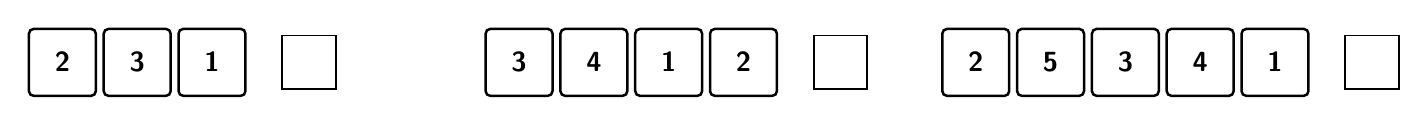
\begin{tikzpicture}[x=1mm,y=1mm]
\draw[line width=0.9pt, fill=white, rounded corners=0.6mm] (0,0) rectangle (8.5,8.5);
\node at (4.25,4.25) {\bfseries 2};
\draw[line width=0.9pt, fill=white, rounded corners=0.6mm] (9.5,0) rectangle (18,8.5);
\node at (13.75,4.25) {\bfseries 3};
\draw[line width=0.9pt, fill=white, rounded corners=0.6mm] (19,0) rectangle (27.5,8.5);
\node at (23.25,4.25) {\bfseries 1};
\draw[line width=0.6pt] (32.17,0.85) rectangle (38.97,7.65);
\draw[line width=0.9pt, fill=white, rounded corners=0.6mm] (58,0) rectangle (66.5,8.5);
\node at (62.25,4.25) {\bfseries 3};
\draw[line width=0.9pt, fill=white, rounded corners=0.6mm] (67.5,0) rectangle (76,8.5);
\node at (71.75,4.25) {\bfseries 4};
\draw[line width=0.9pt, fill=white, rounded corners=0.6mm] (77,0) rectangle (85.5,8.5);
\node at (81.25,4.25) {\bfseries 1};
\draw[line width=0.9pt, fill=white, rounded corners=0.6mm] (86.5,0) rectangle (95,8.5);
\node at (90.75,4.25) {\bfseries 2};
\draw[line width=0.6pt] (99.67,0.85) rectangle (106.47,7.65);
\draw[line width=0.9pt, fill=white, rounded corners=0.6mm] (116,0) rectangle (124.5,8.5);
\node at (120.25,4.25) {\bfseries 2};
\draw[line width=0.9pt, fill=white, rounded corners=0.6mm] (125.5,0) rectangle (134,8.5);
\node at (129.75,4.25) {\bfseries 5};
\draw[line width=0.9pt, fill=white, rounded corners=0.6mm] (135,0) rectangle (143.5,8.5);
\node at (139.25,4.25) {\bfseries 3};
\draw[line width=0.9pt, fill=white, rounded corners=0.6mm] (144.5,0) rectangle (153,8.5);
\node at (148.75,4.25) {\bfseries 4};
\draw[line width=0.9pt, fill=white, rounded corners=0.6mm] (154,0) rectangle (162.5,8.5);
\node at (158.25,4.25) {\bfseries 1};
\draw[line width=0.6pt] (167.18,0.85) rectangle (173.98,7.65);
\end{tikzpicture}
\end{center}

\par\vspace{3pt}\noindent\begin{tikzpicture}[x=1mm,y=1mm]
\draw[black!30, line width=0.4pt] (0,-9) -- (177,-9);
\draw[black!30, line width=0.4pt] (0,-18) -- (177,-18);
\draw[black!30, line width=0.4pt] (0,-27) -- (177,-27);
\draw[black!30, line width=0.4pt] (0,-36) -- (177,-36);
\draw[black!30, line width=0.4pt] (0,-45) -- (177,-45);
\end{tikzpicture}\par
\end{document}
